\documentclass{article}

\usepackage{amsmath}
\usepackage{amssymb}
\usepackage{algorithm}
\usepackage[noend]{algpseudocode}		% for algorithms in pseudo code. Usage: \begin{algorithmic}
\usepackage{subcaption}
\usepackage{tikz}
\usetikzlibrary{decorations.pathmorphing}
\usetikzlibrary{decorations.markings}

\newcommand{\vecl}{\overrightarrow} % long vector for multiple characters
\newcommand{\len}[1]{\left\lVert #1 \right\rVert}
\newcommand{\inta}[1]{\operatorname{int}\left( #1 \right)} % interior angle
\newcommand{\exta}[1]{\operatorname{ext}\left( #1 \right)} % exterior angle

\title{Determining the Convexity of any Polygon}
\author{Abraham Murciano}

\begin{document}
\maketitle

\section{Abstract}

This paper presents and proves the correctness of an algorithm which determines if a sequence of points in three-dimensional space forms a convex polygon or not. We will discuss simple convex and concave polygons as well as complex (self intersecting) polygons, and ultimately even non-planar polygons.

\section{Definitions}

\begin{description}
	\item[Turn between vectors]
		The turn between two three-dimensional vectors \(\vec{u}\) and \(\vec{v}\), which we shall denote henceforth as \(T(\vec{u}, \vec{v}) \in [0, \pi]\), is defined as follows.
		\begin{equation*}
			T(\vec{u}, \vec{v}) = \arccos \left( \frac{\vec{u} \cdot \vec{v}} {\len{\vec{u}} \cdot \len{\vec{v}}} \right)
		\end{equation*}
		For any two vectors there are two angles between them, and the function \(T\) always gives us the smaller of the two.

	\item[Left turn]
		For a vector \(\vec{u}\) and another vector \(\vec{v}\) which is not parallel to \(\vec{u}\) or to \(-\vec{u}\), let \(Q\) be the plane defined by them. If we partition \(\mathbb{R}^3\) into two partitions, one on each face of the plane, and choose one of them as the `top' of the plane and the other as the `bottom', then \(T(\vec{u}, \vec{v})\) is a left turn if \(\vec{u} \times \vec{v}\) points from the plane to the `top' partition.

	\item[Right turn]
		\(T(\vec{u}, \vec{v})\) is a right turn if it is not a left turn. (This means we are treating turns of 0 and of \(\pi\) radians as right turns.)

	\item[Polygon]
		A polygon is a sequence of points (also called vertices) in three-dimensional space where each point is connected to the next by a straight line segment called an edge. There is also an edge between the last and first points. The edges form a closed path.

		Most definitions of a polygon are in fact what we will refer to as a simple polygon, but since we are interested in processing any given sequence of points, and to simplify our language in this paper, we shall extend our definition of a polygon to include any such sequences.

	\item[Planar polygon]
		A planar polygon is a polygon whose vertices all share a common plane.

	\item[Non-planar polygon]
		A non-planar polygon is simply a polygon which is not planar.

	\item[Simple polygon]
		A simple polygon is a planar polygon whose bounding edges do not intersect with one another.

	\item[Convex polygon]
		A polygon is convex if it is simple and all its interior angles are less than \(\pi\) radians.

	\item[Concave polygon]
		A polygon is concave if it is simple and not convex. That is, if it has an interior angle greater than \(\pi\) radians.

	\item[Complex polygon]
		A polygon is complex if it is planar, but not simple. That is, if its edges intersect with each other.

	\item[Turn of a polygon at a vertex]
		If \(A\), \(B\), and \(C\) are three adjacent vertices of a polygon \(P\) such that \(B\) is in between \(A\) and \(C\), the turn of the polygon at the point \(B\) is \(T_P(B) = T(\vecl{AB}, \vecl{BC})\).

		Note, for polygons for which the term `exterior angle' is defined, the turn at a vertex is equal to the absolute value of the exterior angle at that vertex.

	\item[Total turn of a polygon]
		The total turn of a polygon \(P\), is the sum of the turns of all its vertices. We shall use the following shorthand notation to denote this.
		\begin{equation*}
			\sum T_P = \sum_{v \in P} T_P(v)
		\end{equation*}
\end{description}

\begin{figure}[htbp]
	\centering
	\begin{subfigure}{0.25\textwidth}
		\centering
		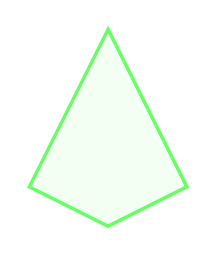
\begin{tikzpicture}
			\filldraw[color=green!60, fill=green!5, very thick] (0, 0) -- (1, -0.5) -- (2, 0) -- (1, 2) -- cycle;
		\end{tikzpicture}
		\caption{Convex}
	\end{subfigure}%
	\begin{subfigure}{0.25\textwidth}
		\centering
		
\begin{tikzpicture}
			\filldraw[color=orange!60, fill=orange!5, very thick] (0, 0) -- (1, 0.5) -- (2, 0) -- (1, 2.5) -- cycle;
		\end{tikzpicture}
		\caption{Concave}
	\end{subfigure}%
	\begin{subfigure}{0.25\textwidth}
		\centering
		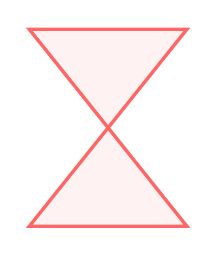
\begin{tikzpicture}
			\filldraw[color=red!60, fill=red!5, very thick] (0, 0) -- (2, 2.5) -- (0, 2.5) -- (2, 0) -- cycle;
		\end{tikzpicture}
		\caption{Complex}
	\end{subfigure}%
	\caption{Examples of different types of polygons.}
	\label{}
\end{figure}

\section{The Algorithm}

We will begin by explaining how the algorithm works, then presenting the algorithm at the end of this section.

\subsection{Input}

The algorithm accepts a sequence of points \(P\) in three-dimensional space. The points represent a polygon formed by constructing an edge between all adjacent vertices in the sequence and an additional edge between the first and last vertices.

\subsection{Output}

The algorithm returns True if the input forms a convex polygon, and False if they form any other type of polygon.

\subsection{Processing}

First, if at least three consecutive points lie consecutively on a single line, the middle points may be removed as they contribute nothing to the polygon and are thus meaningless. The check necessary to do this is simple enough and has been omitted for conciseness. From now on we may assume that any such cases are corrected before any further processing is performed.

The algorithm then boils down to a single check. A sequence of vertices forms a simple convex polygon if and only if the sum of the turns is equal to \(2\pi\). Formally, the algorithm checks if the following equation holds true.

\begin{equation*}
	\sum T_P = 2\pi
\end{equation*}

\subsection{Pseudo Code}

The function \textsc{IsConvex} takes as input a sequence of points \(P\) and returns whether or not the points form a convex polygon.

\begin{algorithm}[htbp]
	\begin{algorithmic}
		\Function{IsConvex}{$P$}
		\State Remove meaningless vertices from \(P\)
		\If{\(|P| < 3\)}
		\Return False
		\EndIf
		\State \(\Sigma := 0\) \Comment{The running sum of the turn.}
		\For{\(i\) from 0 to \(|P| - 1\)}
		\State \(A := P_{i-1 \mod |P|}\) \Comment{The previous point.}
		\State \(B := P_{i}\) \Comment{The current point.}
		\State \(C := P_{i+1 \mod |P|}\) \Comment{The next point.}
		\State \(\Sigma := \Sigma + T(\vecl{AB}, \vecl{BC})\) \Comment{Add the turn at point \(B\).}
		\EndFor
		\State\Return \(\Sigma = 2\pi\)
		\EndFunction
	\end{algorithmic}
\end{algorithm}

\section{Proof of Correctness}

\subsection{Claim}

A sequence of vertices \(P\) forms a convex polygon if and only if the total turn \(\sum T_P\) is equal to \(2\pi\).

In order to prove our claim, we must prove all of the following cases.
\begin{enumerate}
	\item If a polygon is convex then the total turn is equal to \(2\pi\).
	\item If a polygon is concave then the total turn is greater than \(2\pi\).
	\item If a polygon is complex then the total turn is greater than \(2\pi\).
	\item If a polygon is non-planar, then the total turn is greater than \(2\pi\).
\end{enumerate}

\subsection{Proof}

\subsubsection{Convex Polygons Have a Total Turn of Precisely \(2\pi\)}

Suppose a convex polygon \(P\) is drawn on flat ground, and we are standing on one of the edges, facing parallel to the edge with our right foot inside the polygon and our left foot outside. We shall call the direction that we are currently facing the initial direction. Then if we walk forward following the the edges of the polygon, and at each vertex we turn to face the next vertex, eventually we would reach the starting edge again.

At each of the vertices we turned toward the right an amount equal to the exterior angle. It must be the case that we always turn to the right, since every interior angle is less than \(\pi\) radians (by definition of convex), and the inside of the polygon is to our right. See figure \ref{walk-1}.

\begin{figure}[htbp]
	\centering
	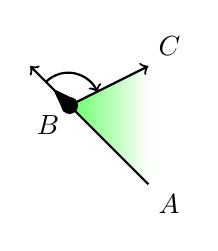
\begin{tikzpicture}
		\shadedraw[->, thick, left color=green!60, right color=white] (0, 0) node[anchor=north west] {\(A\)}
		to (-1, 1) node[anchor=north east] {\(B\)}
		to (0, 1.5) node[anchor=south west] {\(C\)};
		\draw[->, thick] (-1, 1) to (-1.5, 1.5);
		\filldraw (-1, 1) circle (0.1);
		\filldraw (-1.2, 1.2) to (-1.07, 0.93) to (-0.93, 1.07) to cycle;
		\draw[->, thick] (-1.3, 1.3) arc (135:22.5:0.4);
	\end{tikzpicture}
	\caption{Turns at a vertex of a convex polygon are always right turns.}
	\label{walk-1}
\end{figure}

Since we always turned to our right, and we ended up facing the initial direction, and at no other edge or vertex were we facing the initial direction, it must be that in total we turned precisely one rotation, that is, \(2\pi\).

Thus the total amount we turned (\(2\pi\)) must be equal to the sum of the amounts we turned at each vertex (\(\sum T_P\)).

% TODO: continue rewriting notation from here

\subsubsection{A Concave Polygon's Exterior Angles' Sum exceeds \(2\pi\)}

Suppose once again that a polygon is drawn on the ground, but this time let it be concave. Again, suppose we are starting on any edge facing parallel to it with our right foot inside the polygon. This is our initial direction. Suppose we again walk the edges in the same way as we walked the convex polygon.

At some point, we will reach a vertex whose interior angle is greater than \(\pi\) radians (by definition of concave). When this occurs, we will find that the next vertex is on our left hand side, and we will have to turn in that direction (see figure \ref{walk-2}). Since eventually we must reach the starting point and be facing the initial direction, we must at some point turn enough to the right to correct for our leftward deviation. This means that for every interior angle greater than \(\pi\) radians, we will add both the deviation and the correction to the complete turn of \(2\pi\) which we must eventually make.

\begin{figure}
	\centering
	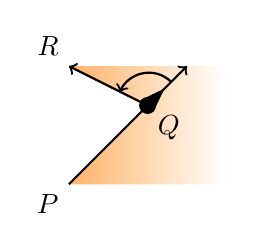
\begin{tikzpicture}
		\shade[left color=orange!60, right color=white] (2, 0) to (0, 0) to (1, 1) to (0, 1.5) to (2, 1.5) to cycle;
		\draw[->, thick] (0, 0) node[anchor=north east] {\(P\)}
		to (1, 1) node[anchor=north west] {\(Q\)}
		to (0, 1.5) node[anchor=south east] {\(R\)};
		\draw[->, thick] (1, 1) to (1.5, 1.5);
		\filldraw (1, 1) circle (0.1);
		\filldraw (1.2, 1.2) to (1.07, 0.93) to (0.93, 1.07) to cycle;
		\draw[->, thick] (1.3, 1.3) arc (45:157.5:0.4);
	\end{tikzpicture}
	\caption{A turn at an vertex \(Q\) of a concave polygon where \(\inta{Q} > \pi\), must be a left turn.}
	\label{walk-2}
\end{figure}%

The deviation at each of these vertices is \(\exta{v}\), and the correction at some future turn must match it. Let \(V' \subset V\) be the set of vertices whose interior angles are greater than \(\pi\). Formally,
\begin{equation}
	V' = \{ v \in V : \inta{v} > \pi \}.
	\label{v-prime}
\end{equation}
Therefore we have the following.
\begin{equation}
	\sum_{v \in V} \exta{v} = 2\pi + 2\sum_{v \in V'} \exta{v}
	\label{ext-concave}
\end{equation}
And since exterior angles are always positive (see definition above), and in the case of every vertex in \(V'\) not equal to zero (otherwise the interior angle would be precisely \(\pi\) contradicting equation \ref{v-prime}), equation \ref{ext-concave} must be strictly greater than \(2\pi\).

\subsubsection{A Complex polygon's Exterior Angles' Sum Exceeds \(2\pi\)}

Suppose for a third time that a polygon is drawn on the ground. This time let the polygon have self intersections and thus be complex. If we were to walk the edges like we did before, we would once again have to end facing the initial direction.

\begin{figure}[htbp]
	\centering
	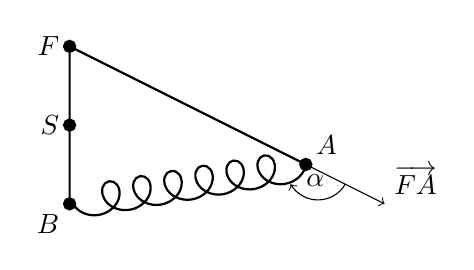
\begin{tikzpicture}
		\filldraw[->, thick] (0, 0) circle (2pt) node[anchor=north east] {\(B\)} to (0, 1) circle (2pt) node[anchor=east] {\(S\)} to (0, 2) circle (2pt) node[anchor=east] {\(F\)} to (3, 0.5) circle (2pt) node[anchor=south west] {\(A\)} node[anchor=120] {\(\alpha\)};
		\draw[->] (3, 0.5) to (4, 0) node[anchor=south west] {\(\vecl{FA}\)};
		\draw[->] (3.5, 0.25) arc (330:210:0.4);
		\draw[thick,decoration={aspect=1, segment length=4mm, amplitude=0.2cm, coil},decorate] (3, 0.5) to (0, 0);
	\end{tikzpicture}
	\caption{Three consecutive points of a complex polygon.}
	\label{walk-3}
\end{figure}

Since we started at a point \(S\) standing on an edge, this edge touches one vertex \(F\) directly in front of us and another vertex \(B\) directly behind us. Then let us single out the next vertex after \(F\), which we will label \(A\). Without loss of generality, we assume this point is on our right from the starting position. See figure \ref{walk-3}, where the curvy edge between \(A\) and \(B\) indicates that the path between them could consist of any number of vertices which could be anywhere on the plane and cause self intersections.

The smallest turn we could make to change direction from facing in the direction \(\vecl{FA}\) at point \(A\) to be arrive at point \(B\) would be \(\alpha = T(\vecl{FA}, \vecl{AB})\) radians (which must be less than \(\pi\) radians, since \(B\) does not lie on the line \(FA\)).

If at point \(A\) we were to deviate from the complex path drawn on the ground and immediately take a turn of \(\alpha\) radians to face \(B\), and subsequently walked straight to point \(B\) and finally back to \(S\), we would form a triangle, whose exterior angles we know to sum up to \(2\pi\).

We may even, on the path from \(A\) to \(B\), turn more than \(\alpha\) radians as with a convex polygon with more than three edges, so long as however much we turn now will eventually be saved when we reach point \(B\) and then make a turn to face the starting point, and thus keeping our exterior angle total equal to \(2\pi\).

However as soon as we turn to the left as with a concave polygon, or turn too far to the right, at least one of which is necessary in order to have self intersections (see figure \ref{self-intersections}), we will have to correct this deviation in the future, therefore we raise our exterior angle total past \(2\pi\).

Thus if a polygon has self intersecting edges, then total turn must be greater than \(2\pi\).

\begin{figure}[htbp]
	\centering
	\begin{subfigure}{0.5\textwidth}
		\centering
		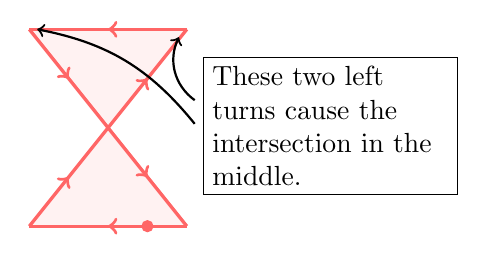
\begin{tikzpicture}
			\fill[fill=red!5] (0, 0) -- (2, 2.5) -- (0, 2.5) -- (2, 0) -- cycle;
			\begin{scope}[very thick,decoration={markings, mark=at position 0.5 with {\arrow{>}}}]
				\draw[color=red!60,  very thick, postaction={decorate}] (0, 0) -- (1, 1.25);
				\draw[color=red!60,  very thick, postaction={decorate}] (1, 1.25) -- (2, 2.5);
				\draw[color=red!60,  very thick, postaction={decorate}] (2, 2.5) -- (0, 2.5);
				\draw[color=red!60,  very thick, postaction={decorate}] (0, 2.5) -- (1, 1.25);
				\draw[color=red!60,  very thick, postaction={decorate}] (1, 1.25) -- (2, 0);
				\draw[color=red!60,  very thick, postaction={decorate}] (2, 0) -- (0, 0);
			\end{scope}
			\node[draw,text width=3cm, anchor=north west] at (2.2, 2.15) {These two left turns cause the intersection in the middle.};
			\filldraw[color=red!60] (1.5, 0) circle (2pt);
			\draw[->, thick, bend left=40] (2.1, 1.6) to (1.9, 2.4);
			\draw[->, thick, bend right=20] (2.1, 1.3) to (0.1, 2.5);
		\end{tikzpicture}
	\end{subfigure}%
	\begin{subfigure}{0.5\textwidth}
		\centering
		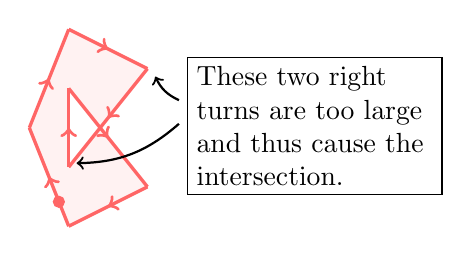
\begin{tikzpicture}
			\fill[fill=red!5] (-0.5, 1.25) -- (0, 2.5) -- (1, 2) -- (0, 0.75) -- (0, 1.75) -- (1, 0.5) -- (0, 0) -- cycle;
			\fill[fill=white] (0, 0.75) -- (0, 1.75) -- (0.4, 1.25) -- cycle;
			\begin{scope}[very thick,decoration={markings, mark=at position 0.5 with {\arrow{>}}}]
				\draw[color=red!60,  very thick, postaction={decorate}] (-0.5, 1.25) -- (0, 2.5);
				\draw[color=red!60,  very thick, postaction={decorate}] (0, 2.5) -- (1, 2);
				\draw[color=red!60,  very thick, postaction={decorate}] (1, 0.5) -- (0, 0);
				\draw[color=red!60,  very thick, postaction={decorate}] (1, 2) -- (0, 0.75);
				\draw[color=red!60,  very thick, postaction={decorate}] (0, 0.75) -- (0, 1.75);
				\draw[color=red!60,  very thick, postaction={decorate}] (0, 1.75) -- (1, 0.5);
				\draw[color=red!60,  very thick, postaction={decorate}] (0, 0) -- (-0.5, 1.25);
			\end{scope}
			\node[draw,text width=3cm, anchor=north west] at (1.5, 2.15) {These two right turns are too large and thus cause the intersection.};
			\filldraw[color=red!60] (-0.125, 0.31) circle (2pt);
			\draw[->, thick, bend left=20] (1.4, 1.6) to (1.1, 1.9);
			\draw[->, thick, bend left=20] (1.4, 1.3) to (0.1, 0.8);
		\end{tikzpicture}
	\end{subfigure}%
	\caption{Self intersections by turning too far right or left.}
	\label{self-intersections}
\end{figure}

\subsubsection{Points which do not share a common plane}

Given a sequence of points in three-dimensional space we may rotate them all in unison in any direction without changing the angles between any edges. Let us then rotate these points so that the plane formed by the first three points is the \(XY\)-plane.

Now suppose we draw this sequence of points on the ground, treating the ground as the \(XY\)-plane, but whenever we encounter a point which does not lie on this plane (which must exist else the points would share a common plane) we raise a hill or dig a ditch in the ground so that we may walk from point to point in a straight line.



\end{document}